%==============================================================================
% Sjabloon onderzoeksvoorstel bachproef
%==============================================================================
% Gebaseerd op document class `hogent-article'
% zie <https://github.com/HoGentTIN/latex-hogent-article>

% Voor een voorstel in het Engels: voeg de documentclass-optie [english] toe.
% Let op: kan enkel na toestemming van de bachelorproefcoördinator!
\documentclass{hogent-article}

% Invoegen bibliografiebestand
\addbibresource{voorstel.bib}

% Informatie over de opleiding, het vak en soort opdracht
\studyprogramme{Professionele bachelor toegepaste informatica}
\course{Bachelorproef}
\assignmenttype{Onderzoeksvoorstel}
% Voor een voorstel in het Engels, haal de volgende 3 regels uit commentaar
% \studyprogramme{Bachelor of applied information technology}
% \course{Bachelor thesis}
% \assignmenttype{Research proposal}

\academicyear{2024-2025} % TODO: pas het academiejaar aan

% TODO: Werktitel
\title{Ontwikkeling en integratie van een Netskope-gebaseerde Data Leakage Prevention (DLP) Oplossing voor vertrouwelijke bedrijfsdata volgens de Belgische regelgeving}

% TODO: Studentnaam en emailadres invullen
\author{Jens Van de Wynckel}
\email{jens.vandewynckel@student.hogent.be}

% TODO: Geef de co-promotor op
\supervisor[Co-promotor]{M. Cremers (Evolane, \href{mailto:mark.cremers@evolane.eu}{mark.cremers@evolane.eu})}



% Binnen welke specialisatierichting uit 3TI situeert dit onderzoek zich?
% Kies uit deze lijst:
%
% - Mobile \& Enterprise development
% - AI \& Data Engineering
% - Functional \& Business Analysis
% - System \& Network Administrator
% - Mainframe Expert
% - Als het onderzoek niet past binnen een van deze domeinen specifieer je deze
%   zelf
%
\specialisation{System \& Network Administrator}
\keywords{Gegevensbescherming, Data Leakage Prevention, Netskope, Belgische regelgeving, PII, PCI, SSE, CASB}
% \keywords{Scheme, World Wide Web, $\lambda$-calculus}

\begin{document}

\begin{abstract}
  De bescherming van vertrouwelijke bedrijfsgegevens vormt een cruciale uitdaging in de digitale wereld, 
  vooral binnen de Belgische juridische context. 
  Deze bachelorproef richt zich op de ontwikkeling en implementatie van een op maat gemaakte Netskope-gebaseerde Data Leakage Prevention (DLP) oplossing, 
  specifiek afgestemd op de Belgische regelgeving. 
  De hoofdonderzoeksvraag is hoe zo'n oplossing effectief kan worden ontworpen en toegepast om zowel te voldoen aan technische en juridische eisen. 
  Met behulp van een combinatie van een literatuurstudie en een praktische Proof of Concept (PoC) worden de mogelijkheden van Netskope beoordeeld in het identificeren, 
  beheersen en voorkomen van datalekken in een realistische testomgeving. Hierbij wordt rekening gehouden met wettelijke kaders zoals de Algemene Verordening Gegevensbescherming (AVG), de NIS2-richtlijn, evenals technische normen zoals PCI DSS en ISO 27001. De PoC zal worden
  uitgevoerd met realistische datascenario's om de oplossing te evalueren. Het onderzoek levert een werkend prototype van een DLP-oplossing op, 
  samen met praktische aanbevelingen voor bedrijven die hun gevoelige data beter willen beschermen. 
  De conclusie laat zien dat een goed uitgewerkte DLP-oplossing niet alleen helpt
  om aan de wetgeving te voldoen, maar ook zorgt voor een betrouwbare bescherming tegen datalekken, zelfs in ingewikkelde bedrijfsomgevingen.
  % Hier schrijf je de samenvatting van je voorstel, als een doorlopende tekst van één paragraaf. Let op: dit is geen inleiding, maar een samenvattende tekst van heel je voorstel met inleiding (voorstelling, kaderen thema), probleemstelling en centrale onderzoeksvraag, onderzoeksdoelstelling (wat zie je als het concrete resultaat van je bachelorproef?), voorgestelde methodologie, verwachte resultaten en meerwaarde van dit onderzoek (wat heeft de doelgroep aan het resultaat?).
\end{abstract}

\tableofcontents

% De hoofdtekst van het voorstel zit in een apart bestand, zodat het makkelijk
% kan opgenomen worden in de bijlagen van de bachelorproef zelf.
%---------- Inleiding ---------------------------------------------------------

% TODO: Is dit voorstel gebaseerd op een paper van Research Methods die je
% vorig jaar hebt ingediend? Heb je daarbij eventueel samengewerkt met een
% andere student?
% Zo ja, haal dan de tekst hieronder uit commentaar en pas aan.

%\paragraph{Opmerking}

% Dit voorstel is gebaseerd op het onderzoeksvoorstel dat werd geschreven in het
% kader van het vak Research Methods dat ik (vorig/dit) academiejaar heb
% uitgewerkt (met medesturent VOORNAAM NAAM als mede-auteur).
% 

\section{Inleiding}%
\label{sec:inleiding}

In dit onderzoek wordt een klantenomgeving ontwikkeld voor Evolane, waarin klantengegevens worden verwerkt en opgeslagen. Deze omgeving zal vertrouwelijke gegevens bevatten die beschermd moeten zijn tegen ongeautoriseerde toegang en datalekken. Data Leakage Prevention (DLP) biedt organisaties de mogelijkheid om hun vertrouwelijke informatie te beschermen tegen datalekken en ongeautoriseerde toegang. Het implementeren van een passende DLP-oplossing moet voldoen aan wettelijke vereisten. In België zijn de bekendste de Algemene verordening gegevensbescherming (AVG) en Payment Card Industry Data Security Standards (PCI DSS) voor betalingsgegevens. Ook de NIS2-richtlijnen en cybersecurity-frameworks zoals het CCB-framework of ISO 27001 kunnen  toegepast worden.
De vraag die centraal staat in dit onderzoek is: “Hoe kan een Netskope-gebaseerde DLP-oplossing ontworpen en geïmplementeerd worden om vertrouwelijke gegevens te beschermen en te voldoen aan de Belgische regelgeving?”. Uit deze hoofdvraag kunnen we een aantal deelvragen afleiden:

\begin{itemize}
    \item Welke mogelijkheden biedt Netskope's Secure Service Edge (SSE) platform voor Data Leakage Prevention (DLP) in de context van vertrouwelijke gegevensbescherming?
    \item Hoe kunnen regelsets en dataclassificatie in Netskope DLP worden afgestemd op de Belgische wetgeving, zoals de AVG en NIS2-richtlijn?
    \item Welke technieken en methoden kunnen worden toegepast om persoonsgegevens (PII) en betalingsgegevens (PCI) effectief te detecteren en te beschermen binnen het Netskope-platform?
    \item Hoe kan een Proof of Concept (PoC) voor Netskope DLP worden opgezet in een testomgeving om de effectiviteit van de oplossing te evalueren?
    \item Welke juridische en technische normen moeten worden meegenomen bij het ontwerpen van een DLP-oplossing voor een Belgische organisatie, en hoe kan Netskope aan deze eisen voldoen?
\end{itemize}

% Waarover zal je bachelorproef gaan? Introduceer het thema en zorg dat volgende zaken zeker duidelijk aanwezig zijn:

% \begin{itemize}
%   \item kaderen thema
%   \item de doelgroep
%   \item de probleemstelling en (centrale) onderzoeksvraag
%   \item de onderzoeksdoelstelling
% \end{itemize}

% Denk er aan: een typische bachelorproef is \textit{toegepast onderzoek}, wat betekent dat je start vanuit een concrete probleemsituatie in bedrijfscontext, een \textbf{casus}. Het is belangrijk om je onderwerp goed af te bakenen: je gaat voor die \textit{ene specifieke probleemsituatie} op zoek naar een goede oplossing, op basis van de huidige kennis in het vakgebied.

% De doelgroep moet ook concreet en duidelijk zijn, dus geen algemene of vaag gedefinieerde groepen zoals \emph{bedrijven}, \emph{developers}, \emph{Vlamingen}, enz. Je richt je in elk geval op it-professionals, een bachelorproef is geen populariserende tekst. Eén specifiek bedrijf (die te maken hebben met een concrete probleemsituatie) is dus beter dan \emph{bedrijven} in het algemeen.

% Formuleer duidelijk de onderzoeksvraag! De begeleiders lezen nog steeds te veel voorstellen waarin we geen onderzoeksvraag terugvinden.

% Schrijf ook iets over de doelstelling. Wat zie je als het concrete eindresultaat van je onderzoek, naast de uitgeschreven scriptie? Is het een proof-of-concept, een rapport met aanbevelingen, \ldots Met welk eindresultaat kan je je bachelorproef als een succes beschouwen?

%---------- Stand van zaken ---------------------------------------------------

\section{Literatuurstudie}%
\label{sec:literatuurstudie}

\subsection{Data Leakage Prevention (DLP)}%

Een DLP-systeem heeft als doel drie soorten gegevens binnen een organisatie te beschermen: data-at-rest, data-in-motion en data-in-use. Data-at-rest verwijst naar statische informatie die is opgeslagen in bedrijfssystemen, zoals documentbeheersystemen, e-mailservers, bestandsservers, netwerkschijven, persoonlijke computers en opslagruimtenetwerken (SANs). Data-in-motion verwijst naar bedrijfsinformatie die zich beweegt binnen het uitgaande netwerkverkeer, zoals e-mails en online verkeer. Data-in-use bestaat uit informatie die medewerkers gebruiken op eindgebruikersapparaten, zoals een bestand kopiëren naar een USB-schijf. De definitie van vertrouwelijkheid binnen een organisatie vraagt om een grondigere analyse. Bepaalde soorten informatie, zoals Persoonlijk Identificeerbare Informatie (PII), waaronder namen, identiteitskaart- en creditcardgegevens, behoren in elke organisatie als vertrouwelijk te worden beschouwd. Deze definitie krijgt echter ingewikkeldere aspecten bij bedrijfsgeheimen en interne communicatie, die vaak onregelmatig zijn. Vertrouwelijke informatie verwijst naar gegevens die binnen de organisatie zijn verzameld en niet algemeen toegankelijk zijn. Een DLP-systeem bevat de mogelijkheid om gevoelige gegevens te herkennen in een of meerdere van de genoemde datatypen.


\subsubsection{PCI en PII}
.
\subsubsection{Gegevensverlies detectie methoden}

Identificatiemiddelen worden gebruikt om gevoelige informatie, zoals PII en PCI, te detecteren. Dit gebeurt op basis van reguliere expressies (regex). Regex is een krachtig hulpmiddel dat DLP helpt specifieke gegevenstypen te herkennen door middel van uitdrukkingen, termen en patronen, zoals \texttt{BE\textbackslash d\{2\}\textbackslash s?\textbackslash d\{4\}\textbackslash s?\textbackslash d\{4\}\textbackslash s?\textbackslash d\{4\}} dat kan dienen voor Belgische IBAN-codes. Hoewel dit patroon effectief is voor standaard IBAN-formaten, kan het worden omzeild door een karakter toe te voegen in de invoer, wat de nood benadrukt van extra controles. 

De aangemaakte identificatie voor confidentiële gegevens moet voldoen aan de volgende richtlijnen:

\begin{itemize}
    \item Vooraf gedefinieerde en aanpasbare patronen voor datadetectie: Het is cruciaal om duizenden vooraf ingestelde regels voor het herkennen van gegevens beschikbaar te hebben en deze te kunnen aanpassen aan de behoeften van de organisatie.
    \item Ondersteuning voor verschillende soorten bestandstypen (Word, Excel, PDF, JPG, PNG, CSV, ZIP en RAR, etc.) en categorieën (afbeeldingen, databases, spreadsheets, etc.).
    \item Ondersteuning voor landspecifieke identificatienummers (IBAN's, postcodes, adressen, nationale identiteitskaarten, IP-adressen, paspoort- en telefoonnummers).
    \item Voldoen aan de wet- en regelgeving.
\end{itemize}

De bescherming van PII en PCI-gegevens vormt een kernaspect van DLP. \textcite{Wason2020CASB} legt de nadruk op het belang van de integratie van Cloud Access Security Brokers (CASB) in cloudomgevingen. CASB biedt organisaties de mogelijkheid om een uitgebreide zichtbaarheid te krijgen in het gebruik van cloudtoepassingen, inclusief goedgekeurde en ongeautoriseerde (shadow IT) diensten. Dit helpt enorm bij het identificeren van waar gevoelige gegevens zich bevinden en hoe ze worden verwerkt.

\subsection{Netskope}%

Netskope heeft zich ontwikkeld tot een vooraanstaande speler in cloudbeveiliging door zijn geavanceerde Secure Service Edge (SSE)-platform. Het levert geïntegreerde CASB- en DLP-mogelijkheden. Volgens \textcite{Riley2018} onderscheidt Netskope zich met functies zoals flexibele regelconfiguraties en realtime-detectie van gevoelige data. \textcite{VanDerWalt2022} identificeren belangrijke aspecten binnen Secure Access Service Edge (SASE) frameworks die nog onvoldoende onderzoek bevatten. Dit combineert netwerk- en beveiligingsdiensten in een cloudgebaseerde omgeving. Deze aspecten zijn onder andere de integratie van verschillende beveiligingscomponenten zoals Secure Web Gateways (SWG), CASB en Zero Trust Network Access (ZTNA). Deze onderdelen dienen samen te werken om een integrale beveiligingsstrategie te creëren. Bovendien is er een toenemende vraag naar het ontwikkelen van API-integraties voor Security Information and Event Management (SIEM)-systemen, zodat gegevens uit verschillende bronnen effectief kunnen worden verzameld en geanalyseerd.
\subsection{Juridisch Kader voor Gegevensbescherming in België}%

De bescherming van persoonlijke en bedrijfsinformatie is een essentieel aspect van de hedendaagse digitale samenleving. Op zowel nationaal als Europees niveau zijn er wettelijke richtlijnen opgesteld om organisaties te ondersteunen bij het garanderen van de vertrouwelijkheid, integriteit en toegankelijkheid van gegevens.

\subsubsection{Algemene Verordening Gegevensbescherming (AVG)}%

Dit onderzoek zal in overeenstemming zijn met de Algemene Verordening Gegevensbescherming (AVG of GDPR) 2016/679 van 27 april 2016 \autocite{eu_avg2016} en de Belgische wet van 30 juli 2018 \autocite{wet_bescherming_2018}.
Volgens de \textcite{eu_avg2016}, overweging (78), moeten passende, technische en organisatorische maatregelen worden genomen om de rechten van natuurlijke personen te beschermen. Deze overweging zorgt ervoor dat persoonsgegevens op een veilige en verantwoorde manier worden verwerkt. Zo'n beveiliging kan gebeuren door middel van standaardinstellingen die erop zijn gericht om risico's in elke fase van de verwerking van gegevens te minimaliseren.
Op 25 juli 2024 publiceerde de Europese Unie haar tweede verslag over de toepassing van de AVG \autocite{eu_avg2024}. Dit rapport legt de nadruk op het feit dat de AVG, ondanks verschillende uitdagingen, een goede basis is voor het veilig en transparant behandelen van persoonsgegevens. 


\subsubsection{Payment Card Industry Data Security Standard (PCI DSS)}%

De Payment Card Industry Data Security Standard (PCI DSS) bestaat uit een reeks richtlijnen en regels die ontworpen zijn voor organisaties die betalingsinformatie en kaartinformatie verwerken, zoals debit-/creditcardnummers, Primary Account Numbers (PAN) en Sensitive Authentication Data (SAD) zoals Card Verification Value (CVV) en magnetische stripgegevens, van alle grote kaartschema’s. Deze standaard is ontwikkeld om de veiligheid van kaartinformatie te garanderen en vereist dat organisaties maatregelen nemen om de gegevens van kaarthouders te beschermen \autocite{Elluri2018}. PCI DSS vereist de implementatie van toegangscontroles, zoals DCS-02 (toegangscontrole tot systemen en gegevens), DCS-07 (beheer van gebruikersidentiteiten en -toegang), en DCS-08 (toegangscontrole tot netwerken en systemen), om de veiligheid van kaartinformatie en de bescherming van kaarthoudergegevens te waarborgen \autocite{Elluri2018}.

\subsubsection{ISO 27001: Informatiebeveiliging}%

Bovendien moet de DLP-oplossing rekening houden met de vereisten van ISO 27001, de internationale norm voor het beheer van informatiebeveiliging. In dit verband bespreken \textcite{Alsanabani2020} de noodzaak van DLP-oplossingen die zowel detectie- als preventieve methoden samenbrengen. De preventieve aanpak probeert datalekken te vermijden door onder andere het gehele confidentiële bestand te versleutelen, toegangscontrole aan te passen en het labelen van de inhoud.

\subsubsection{Nationale en Europese Richtlijnen}%

Buiten de Belgische wetgeving zijn er ook tal van Europese richtlijnen en nationale standaarden die een belangrijke rol hebben in de bescherming van bedrijfsdata. Hierbij kan gedacht worden aan de Algemene Verordening Gegevensbescherming (AVG), de EU Cybersecurity Act en belangrijke Europese richtlijnen, waaronder de NIS2-richtlijn. Deze richtlijnen worden verder uitgebreid met specifieke normen, zoals de PCI DSS voor betalingsgegevens en internationale normen, zoals ISO 27001 voor de beveiliging van informatie. 
De NIS2-richtlijn (Richtlijn (EU) 2022/2555), die op 16 januari 2023 is aangenomen door de \cite{nis2directive}, heeft als doel de cyberbeveiliging binnen de EU te versterken door een hoog niveau van beveiliging te waarborgen voor netwerken en informatiesystemen. Artikel 21 van de NIS2-richtlijn richt zich op de beveiliging van netwerken en informatiesystemen en legt de verplichting op aan lidstaten om ervoor te zorgen dat aanbieders van essentiële en belangrijke diensten passende technische en organisatorische maatregelen nemen. maatregelen die over het DLP-systeem kunnen gaan, zijn onder andere: 

\begin{itemize}
    \item Risicoanalyse (lid 2, punten a en e): Organisaties moeten een risicobeheerproces implementeren dat hen in staat stelt om risico's voor de beveiliging van netwerken en informatiesystemen te identificeren, te evalueren en te beheersen.
    \item Encryptie en toegangscontroles (lid 2, punten h en i): Het gebruik van encryptie, toegangscontroles en regelmatige beveiligingstests en audits.
    \item Incidentenbehandeling (lid 2, punt b): Organisaties moeten procedures en mechanismen hebben voor het detecteren, melden en reageren op beveiligingsincidenten.
    \item Bewustwording en training (lid 2, punt g): Opleidingen en bewustwordingsprogramma's om medewerkers te informeren over goede cyberhygiëne en risicomanagement. \autocite{nis2directive} Het DLP-systeem van Netskope staat in voor het trainen van de eindgebruiker, mocht deze iets foutief doen.
\end{itemize}

De studie van \textcite{Nayak2020} geeft een uitgebreid overzicht van systemen voor het detecteren en voorkomen van datalekken, inclusief de indeling van systemen op basis van de status van de gegevens (data-at-rest, data-in-motion, data-in-use) en de detectietechnieken. Dit overzicht zal gebruikt worden voor het ontwikkelen van regex-gebaseerde regels in DLP-oplossingen. De studie legt de nadruk op het feit dat datalekken zowel onvoorzien als opzettelijk kunnen optreden en geeft uitdagingen aan, zoals het identificeren van gevoelige informatie, het balanceren van de detectienauwkeurigheid en de integratie van geavanceerde methodologieën.

% \subsubsection{Gegevensoverdracht en internationale implicaties}%

\subsubsection{Andere relevante wetgeving}%

De onderstaande tabel bevat de belangrijkste wettelijke richtlijnen en uitspraken die relevant zijn voor het ontwerp en de implementatie van een Data Leakage Prevention-oplossing voor Belgische bedrijven.

\begin{figure}
    \centering
    % \includegraphics[width=.2\textwidth]
    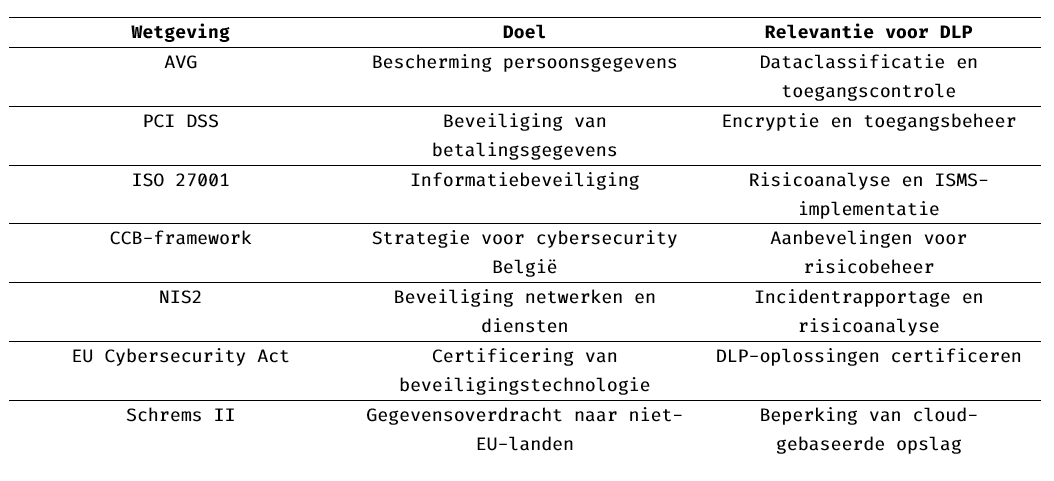
\includegraphics[scale=0.50]
    {img/overzicht.png}
    \caption{\label{fig:overzicht}Overzicht van de belangrijkste wettelijke richtlijnen en uitspraken voor DLP-oplossingen in België.}
  \end{figure}

% Hier beschrijf je de \emph{state-of-the-art} rondom je gekozen onderzoeksdomein, d.w.z.\ een inleidende, doorlopende tekst over het onderzoeksdomein van je bachelorproef. Je steunt daarbij heel sterk op de professionele \emph{vakliteratuur}, en niet zozeer op populariserende teksten voor een breed publiek. Wat is de huidige stand van zaken in dit domein, en wat zijn nog eventuele open vragen (die misschien de aanleiding waren tot je onderzoeksvraag!)?

% Je mag de titel van deze sectie ook aanpassen (literatuurstudie, stand van zaken, enz.). Zijn er al gelijkwaardige onderzoeken gevoerd? Wat concluderen ze? Wat is het verschil met jouw onderzoek?

% Verwijs bij elke introductie van een term of bewering over het domein naar de vakliteratuur, bijvoorbeeld~\autocite{Hykes2013}! Denk zeker goed na welke werken je refereert en waarom.

% Draag zorg voor correcte literatuurverwijzingen! Een bronvermelding hoort thuis \emph{binnen} de zin waar je je op die bron baseert, dus niet er buiten! Maak meteen een verwijzing als je gebruik maakt van een bron. Doe dit dus \emph{niet} aan het einde van een lange paragraaf. Baseer nooit teveel aansluitende tekst op eenzelfde bron.

% Als je informatie over bronnen verzamelt in JabRef, zorg er dan voor dat alle nodige info aanwezig is om de bron terug te vinden (zoals uitvoerig besproken in de lessen Research Methods).

% % Voor literatuurverwijzingen zijn er twee belangrijke commando's:
% % \autocite{KEY} => (Auteur, jaartal) Gebruik dit als de naam van de auteur
% %   geen onderdeel is van de zin.
% % \textcite{KEY} => Auteur (jaartal)  Gebruik dit als de auteursnaam wel een
% %   functie heeft in de zin (bv. ``Uit onderzoek door Doll & Hill (1954) bleek
% %   ...'')

% Je mag deze sectie nog verder onderverdelen in subsecties als dit de structuur van de tekst kan verduidelijken.

%---------- Methodologie ------------------------------------------------------
\section{Methodologie}%
\label{sec:methodologie}

De daadwerkelijke studie naar Data Leakage Prevention (DLP) oplossingen zal theoretisch starten, gevolgd door een praktische Proof of Concept (PoC) in een testomgeving die Evolane zal geven. Hiervoor zal een grondige documentatie opgesteld worden.

\subsection{Omgeving}%

De omgeving zal dienen als testomgeving. Dit zal intern in het bedrijf opgesteld worden. Een licentie van Netskope zal dienen om de DLP-service op te zetten. Deze omgeving zal alle soorten data bevatten (data-in-use, data-in-motion, data-at-rest)  Confidentiële en niet-confidentiële bestanden/data zullen dienen om uit te maken of de DLP-service al het juiste kan identificeren en verdere verwerking kan tegenhouden. De data bestaat vooral uit persoonlijk identificeerbare informatie (PII) en betalingsgegevens (PCI) die verplicht beveiligd moeten zijn door al de opgegeven wetten, richtlijnen of uitspraken (AVG, PCI DSS, ISO 27001, NIS2, Schrems II,..).  Zelf aangemaakte gebruikers met verschillende rechten zullen hierop data doorsturen en verwerken. De testomgeving simuleert realistische klantenscenario’s om te beoordelen hoe effectief deze oplossing werkt.

% \subsection{Regex}%

% !!!!!!!!!!!!!!!!!!!!!!!!!!
% \subsection{Testen}%
% !!!!!!!!!!!!!!!!!!!!!!!!!!

% Hier beschrijf je hoe je van plan bent het onderzoek te voeren. Welke onderzoekstechniek ga je toepassen om elk van je onderzoeksvragen te beantwoorden? Gebruik je hiervoor literatuurstudie, interviews met belanghebbenden (bv.~voor requirements-analyse), experimenten, simulaties, vergelijkende studie, risico-analyse, PoC, \ldots?

% Valt je onderwerp onder één van de typische soorten bachelorproeven die besproken zijn in de lessen Research Methods (bv.\ vergelijkende studie of risico-analyse)? Zorg er dan ook voor dat we duidelijk de verschillende stappen terug vinden die we verwachten in dit soort onderzoek!

% Vermijd onderzoekstechnieken die geen objectieve, meetbare resultaten kunnen opleveren. Enquêtes, bijvoorbeeld, zijn voor een bachelorproef informatica meestal \textbf{niet geschikt}. De antwoorden zijn eerder meningen dan feiten en in de praktijk blijkt het ook bijzonder moeilijk om voldoende respondenten te vinden. Studenten die een enquête willen voeren, hebben meestal ook geen goede definitie van de populatie, waardoor ook niet kan aangetoond worden dat eventuele resultaten representatief zijn.

% Uit dit onderdeel moet duidelijk naar voor komen dat je bachelorproef ook technisch voldoen\-de diepgang zal bevatten. Het zou niet kloppen als een bachelorproef informatica ook door bv.\ een student marketing zou kunnen uitgevoerd worden.

% Je beschrijft ook al welke tools (hardware, software, diensten, \ldots) je denkt hiervoor te gebruiken of te ontwikkelen.

% Probeer ook een tijdschatting te maken. Hoe lang zal je met elke fase van je onderzoek bezig zijn en wat zijn de concrete \emph{deliverables} in elke fase?

%---------- Verwachte resultaten ----------------------------------------------
\section{Verwacht resultaat, conclusie}%
\label{sec:verwachte_resultaten}

Dit onderzoek zal een volledig uitgewerkt Proof of Concept (PoC) opleveren van een Netskope-gebaseerde DLP-oplossing, die is ontworpen om vertrouwelijke gegevens, zoals PII- en PCI-gegevens, te beschermen volgens de Belgische wetgeving. De PoC zal datalekken identificeren en beschermen in een realistische testomgeving die door de klant 'Evolane' mede opgezet zal worden. De vertrouwelijke data zullen in alle mogelijke datatypen voorkomen, zoals data-in-use, data-in-motion en data-at-rest. De oplossing zal gericht zijn op het voorkomen van datalekken die kunnen optreden bij het verwerken en verplaatsen van gevoelige gegevens, zowel binnen als buiten de organisatie.
De proof-of-concept zal een geconfigureerd DLP-platform opleveren dat PII- en PCI-gegevens kan identificeren en beschermen volgens de vooraf ingestelde parameters. Deze parameters zullen voldoen aan klant-specifieke dataclassificaties en zullen worden gevalideerd aan de hand van specifieke testscenario's. Het resultaat van deze tests wordt gepresenteerd in een evaluatierapport, dat de effectiviteit van de oplossing evalueert.
Daarnaast zal het onderzoek aanbevelingen doen over hoe organisaties de Netskope DLP-oplossing kunnen implementeren om te voldoen aan zowel technische als juridische normen. Het verwacht resultaat omvat een succesvolle implementatie van een DLP-oplossing die effectief de risico's van datalekken vermindert.

% Hier beschrijf je welke resultaten je verwacht. Als je metingen en simulaties uitvoert, kan je hier al mock-ups maken van de grafieken samen met de verwachte conclusies. Benoem zeker al je assen en de onderdelen van de grafiek die je gaat gebruiken. Dit zorgt ervoor dat je concreet weet welk soort data je moet verzamelen en hoe je die moet meten.

% Wat heeft de doelgroep van je onderzoek aan het resultaat? Op welke manier zorgt jouw bachelorproef voor een meerwaarde?

% Hier beschrijf je wat je verwacht uit je onderzoek, met de motivatie waarom. Het is \textbf{niet} erg indien uit je onderzoek andere resultaten en conclusies vloeien dan dat je hier beschrijft: het is dan juist interessant om te onderzoeken waarom jouw hypothesen niet overeenkomen met de resultaten.



\printbibliography[heading=bibintoc]

\end{document}